% !TEX encoding = UTF-8 Unicode
\documentclass[11pt,a4paper]{report}		                                   

\usepackage{graphicx}
\usepackage{a4}
\usepackage[T1]{fontenc}
\usepackage[utf8]{inputenc}
\usepackage[ngerman]{babel}

\usepackage{wrapfig}  
\usepackage{acronym}
\usepackage{enumitem}
\usepackage[ampersand]{easylist}

\usepackage{listings}
\usepackage{color}
\usepackage{graphicx}
\usepackage{float}

\usepackage{caption}
\captionsetup{margin=8pt,font=footnotesize,format=hang}

\usepackage{url}

%Platzierung von Tabelle in Kapitel erzwingen 
\usepackage[section]{placeins}

%Tabellen
\usepackage{booktabs}
\usepackage[table,xcdraw]{xcolor}

\usepackage{chngcntr}
\counterwithout{figure}{chapter} %Kapitelübergreifende Bildnummerierung
\counterwithout{table}{chapter} %Kapitelübergreifende Tabellennummerierung

%Listings
\usepackage{listings} 
\lstset{
	  numbers=none,
	  numberstyle=\tiny,
	  numbersep=5pt,
	  captionpos=b,
	  showstringspaces=false,
	  basicstyle=\footnotesize\ttfamily,
	  numberbychapter=false%TODO
	  }
\lstset{language=Java}
\renewcommand{\lstlistingname}{Auflistung}
\renewcommand{\lstlistlistingname}{Auflistungen}
 
%Baumstruktur
\usepackage{tikz}
\usetikzlibrary{arrows,shapes,positioning,shadows,trees}

\tikzset{
	basic/.style = {draw, text width=2m, drop shadow, font=\sffamily, rectangle},
	root/.style = {basic, rounded corners=2pt, thin, align=center,
		fill=green!30},
	level 2/.style = {basic, rounded corners=6pt, thin,align=center, fill=green!60,
		text width=8em},
	level 3/.style = {basic, thin, align=left, fill=pink!60, text width=6.5em}
}

%Kapitelüberschriften
 \usepackage{fancyhdr} %Fancy Header
 \pagestyle{fancy}
 \fancyhead{}  
 \fancyhead[RE,RO]{\normalsize\sffamily \thechapter \ \leftmark} 
\cfoot{ \thepage}
 \renewcommand{\headrulewidth}{0pt}  
 \renewcommand{\chaptermark}[1]{\markboth{#1}{}}
 
 % set colors for links and URLs
 \usepackage[
 colorlinks=true,
 urlcolor=black,
 linkcolor=black,
 citecolor=black
 ]{hyperref}
 
%Fußnoten
\usepackage{scrextend} %Formatierung der Fuߟnoteneinträge
\deffootnote{1.5em}{1em}{ %Fußnoten Formatierung
	\makebox[1.5em][l]{\thefootnotemark}} % [l]-->Links

%handle subsections
\setcounter{secnumdepth}{3}
\setcounter{tocdepth}{3}

% Literatur - Achtung alphadin file angepasst!
\bibliographystyle{alphadin}




%Eigene Commands, falls gewuenscht
\newcommand{\umbruch}{\\ \noindent}		%Zeilenumbruch
\newcommand{\absatz}{\\ \\ \noindent}	%Absatz ohne einrücken
\newcommand{\extra}[1]{\emph{#1}} 		%Fremdworte, Englische Worte, ... kursiv

\renewcommand\lstlistingname{Quelltext} % Change language of section name

\newcommand{\thema}{E-Bildung}
\newcommand{\untertitel}{Die digitalisierung des Schulunterrichts}
\newcommand{\autoren}{Marco Boxler, Lukas Groß, Tarek Büchner}
\newcommand{\abgabedatum}{30.06.2018}
\newcommand{\arbeitsTyp}{Ausarbeitung}

\begin{document}

\begin{titlepage}

\vspace*{-3.5cm}

\begin{flushleft}
\hspace*{-1cm} 
\includegraphics[width=15.7cm]{front/htwg-logo.png}
\end{flushleft}

\vspace{2.5cm}

\begin{center}
	\huge{
		\textbf{\thema} \\[3cm]
	}
	\Large{
		\textbf{\untertitel}} \\[6.5cm]
	\Large{
		\textbf{\autoren}} \\[3cm]
	\large{
		\textbf{Konstanz, \abgabedatum} \\[1.8cm]
	}
	
	\Huge{
		\textbf{{\sf \arbeitsTyp}}
	}
\end{center}

\end{titlepage}


\pagenumbering{gobble}
\tableofcontents
	\thispagestyle{empty}
\clearpage 
\pagenumbering{arabic}

% So werden Kapitel inkludiert
% \include{chapters/chapterName}
% !TEX encoding = UTF-8 Unicode
\chapter{Minecraft in Education}

\section{Einleitung und Motivation}

In unserer heutigen Gesellschaft wird Medienkompetenz immer wichtiger. Sehr viele Berufe benötigen ein hohes Wissen im Bereich von Fachanwendungen (Office, Adobe etc.) für den Computer. 
Aber auch Menschen mit Berufen, ohne den Einsatz von Computern, werden in Ihrer Freizeit und Umgebung immer mehr von der Digitalisierung betroffen.
Smartphones und Tablets sind mittlerweile allgegenwärtig. An den Hochschulen hat fast jeder Student einen Notebook oder ein Tablet.
Bücher werden durch E-Books ersetzt und Vorlesungs-Unterlagen sind nur noch digital verfügbar. Deshalb ist es umso wichtiger, die nächsten Generationen auf diesen Wandel vorzubereiten. 
Ziel muss es sein, den Umgang mit Medien wie Computern von Klein auf zu üben.

Um dies zu erreichen, soll Wissen spielerisch vermitteln und die bisherigen Medien im Schulsystem durch die neue Generation der Lernspiele erweitert werden.
Bisher waren Lernspiele häufig technisch und spielerisch veraltet (im Vergleich zu modernen Computerspielen) und als Einzelspieler-Spiele konzipiert. Moderne Lernspiele setzten hier auf den Online/Mehrspieler-Aspekt um Gruppenarbeit zu fördern und Schulen miteinander zu vernetzen.

Internationale Unternehmen wie Google, Microsoft und Apple haben erkannt wie wichtig diese neue Form der Lernspiele ist und fördern diese im Schulbereich.
Ein Projekt, auf welches in diesem Kapitel näher eingegangen wird, ist Minecraft in Education.

\section{Projekt Minecraft in Education}

Im Jahr 2009 wurde Minecraft (Version old aplha rd-132211) das erste mal vom
Studio Mojang veröffentlicht. Hauptentwickler war Markus Notch Persson. Zu Beginn wurde Minecraft
ausschließlich über die eigene Webseite des Studios vertrieben und löste bereits nach kurzer Zeit,
einen Hype in der Spielwelt aus. 2014 wurde das Studio von Microsoft aufgekauft. Darauf folgte eine Minecraft Version für die mobile Plattformen (Android, IOS) und eine für Windows 10.
\cite{WikiMinecraft}\cite{HeiseMicrosoft}

Minecraft ist ein Computerspiel ohne direktes Spielziel, man spricht von einem \textbf{Sandbox}-Spiel.
Der Spieler übernimmt die Kontrolle über einen Avatar und kann mithilfe von würfelförmigen Blöcken,
in einer 3D-Welt, Konstruktionen erschaffen oder vorhandene bearbeiten. Der Kreativität selbst,
sind dabei kaum Grenzen gesetzt, es gibt eine Vielzahl verschiedener Blockarten mit unterschiedlichen
Eigenschaften. So gibt es Blöcke die physikalisch Korrekt von der Schwerkraft beeinflusst werden,
andere die wiederum in der Luft schweben können und manche die sich wie Flüssigkeiten verhalten.
\cite{WikiMinecraft}

Ein weiterer Grund für die fast unendlichen Möglichkeiten, ist die Erweiterbarkeit des Spiels durch
,von Spielern erstellten, Modifikationen (In der Szene Mods genannt). Mit diesen Erweiterungen ist es
möglich, bis auf das Blocksystem, alle Bereiche des Spieles anzupassen. Einem Weltraumspiel oder einer
Dreidimensionalen Murmelbahn steht nichts im Wege. Neue Arten von Blöcken mit neuen Eigenschaften lassen
sich dabei ebenso einfügen. 

Eine dieser Modifikationen ist das Projekt Minecraft in Education, welches
von Mojang AB und Microsoft Studios gemeinsam entwickelt und Vertrieben wird, mit dem Ziel Minecraft für die Verwendung im Klassenraum anzupassen. \cite{GamepediaMinecraft}

\begin{figure}[ht]
	\centering
	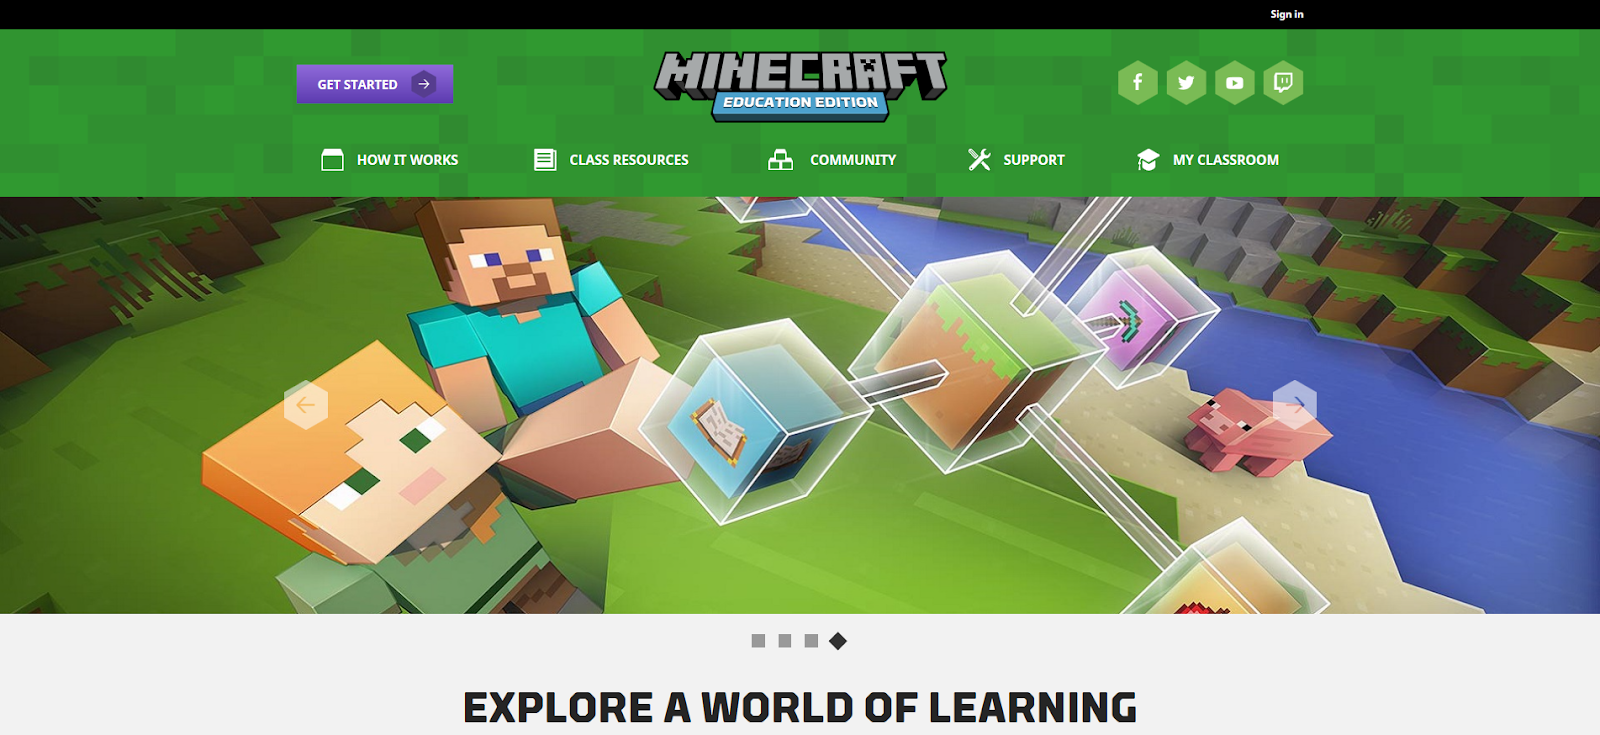
\includegraphics[width=\textwidth,height=\textheight,keepaspectratio]{images/Minecraft.png}
	\caption{Projekt Minecraft in Education \cite{HomepageMinecraftEducation}}
	\label{projectMinecraft}
\end{figure}

Die erste Version wurde am 1.November 2016 veröffentlicht und wird bisher von 2 Millionen Nutzern ausprobiert/genutzt, laut Microsoft.

\section{Der virtuelle Klassenraum}

Mit virtuellen Klassenraum ist an dieser Stelle das Treffen der Schüler und Lehrer in einer virtuellen Umgebung, auch Spielwelt genannt, gemeint. Ein Klassenraum bzw. eine Spielwelt kann je nach Einstellungen beliebig viele Teilnehmer haben. Als Richtwert werden 30 Spieler angegeben. Diese Klassenräume können entweder direkt mit dem Internet verbunden werden und damit Schulübergreifende Projekte ermöglichen oder lokal für die jeweilige Schule konfiguriert sein.

Innerhalb dieser Welten gibt es viele wichtige Konzepte, die in diesem Abschnitt erläutert werden.

\subsection{Spielwelt}

Die Spielwelt ist der Ort an dem sich die Schüler und Lehrenden treffen um den Unterricht abzuhalten.
Kommuniziert wird dabei entweder per Textchat oder Sprachchat. Jeder Teilnehmer hat zusätzlich eine eigene Spielwelt. Dadurch ist es möglich Gruppenarbeiten durchzuführen, in dem man sich entweder in der Spielwelt der Klasse oder des Schülers trifft.

Die Spielwelten können sehr unterschiedliche Formen annehmen. Nachfolgend ist die virtuelle Version des Globe Theatre in London, für den Geschichtsunterricht, abgebildet.

\begin{figure}[ht]
	\centering
	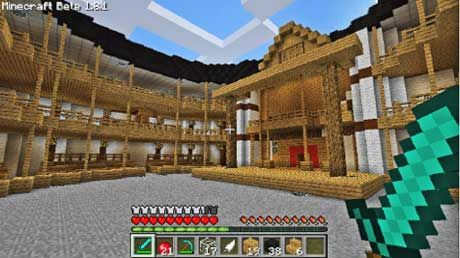
\includegraphics[width=\textwidth,height=\textheight,keepaspectratio]{images/GlobeTheatreLondon.png}
	\caption{Globe Theatre London als virtuelle Version \cite{EdutopiaIdeas}}
	\label{globeTheatreLondon}
\end{figure}

Durch diese virtuellen Schauplätze kann das vermittelte Wissen in Geschichte anschaulich dargestellt werden. Der Schüler erhält dadurch nicht nur die Möglichkeit, Schauplätze zu besuchen, sondern erhält auch Eindrücke wie z.B. die Größe des Kolosseums in Rom. \cite{EdutopiaIdeas}

Diese Information lässt sich mit Worten, Bildern oder Zeichnungen alleine nur schwer vermitteln. Dies ergänzt somit sinnvoll die eingesetzten Medien im Unterricht.

\subsection{Kameras}

Kameras sind Objekte, die ein Spieler mit sich führt. Sie werden verwendet um den Lernfortschritt oder Entdeckungen festzuhalten. Dies ist sehr wichtig, da nicht nur der Spaß am Spielen im Vordergrund steht, sondern auch die Überprüfbarkeit der Leistung durch den Lehrer. Nach dem Unterricht, kann damit zu einem beliebigen Zeitpunkt, das Ergebnis eines Schülers betrachtet und bewertet werden.

\subsection{Blöcke}

Eine Spielwelt besteht aus Blöcken mit unterschiedlichen Eigenschaften. Diese können unter anderem verwendet werden um die Spielwelt zu begrenzten, Flüssigkeiten darzustellen oder Gravitation zu simulieren.

Mit dem \textbf{Redstone}-Block können beispielsweise elektrische Schaltungen entworfen werden. Dazu nimmt der Schüler mehrere Blöcke und verknüpft sie miteinander. Über einen Schalter werden diese anschließend unter Strom gesetzt und das Ergebnis wird sichtbar, wie nachfolgend dargestellt.

\begin{figure}[ht]
	\centering
	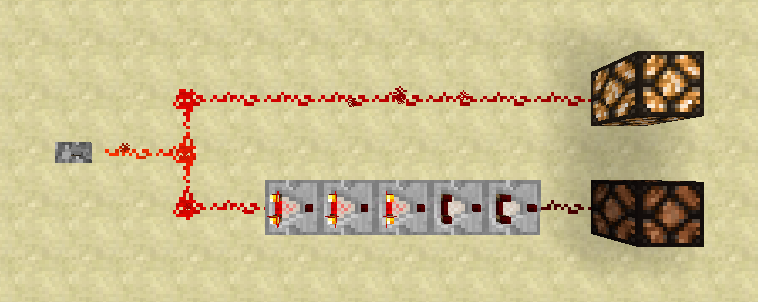
\includegraphics[width=\textwidth,height=\textheight,keepaspectratio]{images/RedstoneSignalverzoegerer.png}
	\caption{Signalverzögerer mit \textbf{Redstone} \cite{GamepediaMinecraft}}
	\label{redstoneSignalDelay}
\end{figure}

Die dargestellte Schaltung verzögert ein Signal. Das \textbf{Redstone} sind die roten Linien, welche unter Storm gesetzt werden. Der etwas hellere Block oben rechts, stellt eine Lampe dar, die leuchtet. Unten auf der rechten Seite befindet sich eine Lampe, die noch aus ist und verzögert angeschaltet wird.
Dies ist nur ein mögliches Szenario, mit \textbf{Redstone} lassen sich beliebige Schaltungen simulieren.
Dadurch kann dem Schüler wissen im Bereich Technik, Physik und auch Programmieren vermittelt werden.

Damit die Schüler nicht alle Bereiche der Spielwelt verändern können und um Chaos zu verhindern, kann der Lehrende die sogenannten \textbf{Deny} und \textbf{Allow}-Blöcke verwenden. Mit einem Allow-Block, wird ein bestimmtes Gebiet zum Bearbeiten freigegeben, mit dem Deny-Block hingegen verboten. Dies ist wichtig um den Schülern Grenzen festzulegen.
Die folgenden Abbildung zeigt einen Allow- und Deny-Block (Hellbrauner und grauer Block).

\begin{figure}[ht]
	\centering
	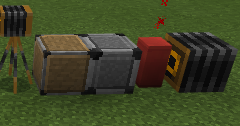
\includegraphics{images/AllowAndDenyBlocks.png}
	\caption{Allow und Deny Blöcke \cite{GamepediaMinecraft}}
	\label{allowDenyBlocks}
\end{figure}

\subsection{NPCs}

Ein wichtiges Element im virtuellen Klassenraum sind die sogenannten NPCs (Non-player characters).
Darunter versteht man Figuren, in der virtuellen Welt, die nicht selbst vom Lehrer gesteuert werden und Verwendung finden, um dem Spieler Anleitung oder Hinweise zu geben. Dadurch kann ein Lehrer wichtige Anmerkungen für die Schüler geben, die zu jedem Zeitpunkt abgerufen werden können, der Lehrer selbst muss nicht anwesend sein.
Dies kann eingesetzt werden, um noch einmal eine Zusammenfassung des Unterrichtstoffes zu geben oder die Aufgabenstellung zu wiederholen. Nachfolgend zeigt, wie ein NPC in Minecraft aussehen kann.

\begin{figure}[ht]
	\centering
	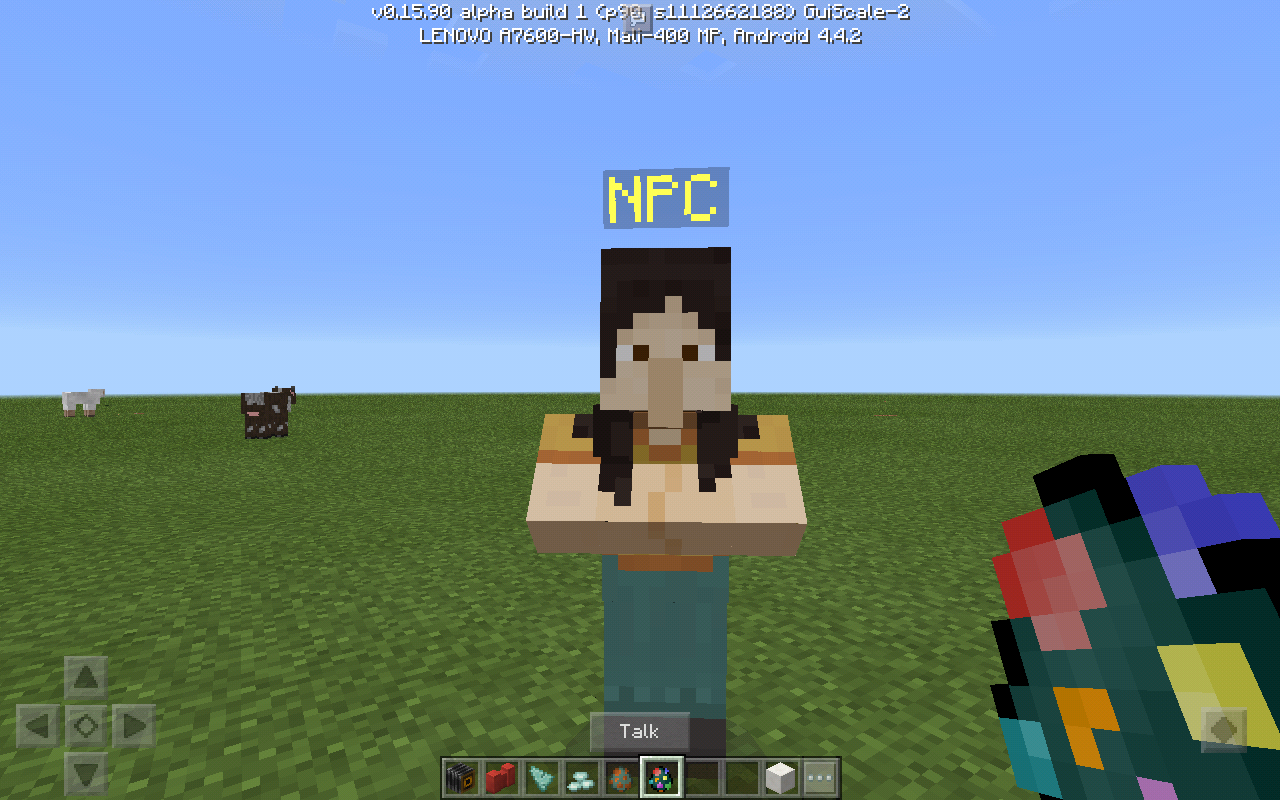
\includegraphics[width=\textwidth,height=\textheight,keepaspectratio]{images/NPC.png}
	\caption{Ein NPC \cite{GamepediaMinecraft}}
	\label{npc}
\end{figure}

\subsection{Kurse}

Ein Kurs meint eine abgeschlossene Lektion, innerhalb eines Faches. Technisch gesehen, ein Wiederherstellungspunkt einer Spielwelt, zu einem bestimmten Zeitpunkt. Diese können separat abgespeichert und jederzeit kann darauf zugegriffen werden. Dies ist ein wichtige Funktion von Minecraft in Education, da es erlaubt, Kursinhalte zwischen Schule und anderen Einrichtungen zu tauschen.

\section{Vernetzung von Schulen}

Nach dem im vorherigen Abschnitt ausführlich der Aufbau des virtuellen Klassenraums beschrieben wird, legt dieser Abschnitt den Fokus auf dem praktischen Nutzen bei der Vernetzung von Schule und sonstigen Einrichtungen.
Immer häufiger liest man vom Fachkräftemangel unter anderem im Schulsystem. Hier bietet Minecraft in Education mit seinen Online-Funktionalitäten eine große Chance. Ein Lehrer oder Tutor muss nicht länger an einer Schule vor Ort sein. Er kann von Zuhause oder seinem Arbeitsplatz, das virtuelle Klassenzimmer betreten und seinen Unterricht halten. Dadurch können starke Synergien zwischen spezialisierten Schulen gebildet und Wissen transferiert werden.
Außerdem können, wie zuvor unter Kurse beschrieben, Lehrinhalte aufgezeichnet und ausgetauscht werden.
Die Idee dahinter ist, eine Länderübergreifende Wissensdatenbank zu schaffen.

Neben dem Transfer von Wissen an Schülern, wird auch die Chance geboten, IT Wissen an anderen Schulen weiterzugeben. Dies ist insbesondere wichtig, da auch die Ansprüche an die Lehrkräfte durch die immer stärker werdende Digitalisierung steigen. Hierfür können Kurs erstellt oder zumindest Kontakt über die virtuelle Welt hergestellt werden. Ziel sollte es sein, auch dort den Austausch zwischen den Schulen zu fördern.

\section{Auswirkungen auf das Lernverhalten?}

Eine der spannenden Fragen zu diesem Thema lautet: Wie wirkt sich der Einsatz von Lernspielen auf das Lernverhalten aus?

Pauschal lässt sich diese Frage nicht beantworten. Viele Faktoren, wie Spaß am spielerischen Lernen oder Vorkenntnisse eines Schülers, spielen eine große Rolle. Was aber gesagt werden kann, ist das die spielerisch Herangehensweise an komplexe Themen, wie in der Mathematik, vielen Schülern die Angst nimmt.

Ebenso macht vielen Kindern die Arbeit in der Gruppe Spaß und motiviert sie. Mit Freunden und Klassenkameraden zu Spiele und auch mal Blödsinn zu machen, ist wichtig für die Motivation in der Gruppe. Hier sollten die Lehrenden auf ein gutes Gleichgewicht achten. Durch das frühe arbeiten in Teams, wird die Teamfähigkeit geübt was später für das Studium und den beruflichen Alltag entscheidend ist.

Auch der Umgang mit den eigenen Daten kann vermittelt werden, in dem den Schülern gezeigt wird, welche Daten gesammelt und gespeichert werden. Dies kann auf Beispiele in der realen Welt, wie Facebook und Google übertragen werden. Es ist sehr wichtig, junge Menschen für dieses Thema zu sensibilisieren.

\section{Gibt es Risiken?}

Neben den positiven Aspekten gibt es auch Gewisse Risiken beim Einsatz von Minecraft in Education und anderen Lernspielen.

Nicht alle Schüler sind geübt im Umgang mit Computern und hier muss der Lehrende ein gutes Gleichgewicht finden zwischen den Vorkenntnissen der Schüler. Falls der Unterschied zu groß ist, sollte die Klasse aufgeteilt werden.

Viele Schüler kennen in der heutigen Zeit das Internet und dessen Anonymität. Deshalb ist es wichtig, auf die Kommunikation der Schüler untereinander zu achten. Nicht Jeder ist sich bewusst, wie sich geschriebene Worte auf andere Menschen auswirken können. Dies muss auch erlernt werden. Eine Hilfe bietet hier sicher die Möglichkeit den Sprachchat zu verwenden. Je nach Kenntnisstand kann auch ein Schimpfwort-Filter eingesetzt werden. Durch das Aufzeichnen der Unterrichtstunden, kann das Kommunikationsverhalten der Schüler nachträglich überprüft werden.

\section{Für wen eignet sich Minecraft in Education?}
Minecraft in Education kann für verschiedene Altersgruppen eingesetzt werden. Es gibt je nach Schulsystem für Kinder (Grundschulen) bis Jugendlichen (Gymnasien) ein breites Spektrum an Anwendungsmöglichkeiten. Generell sollte es zur jeweiligen Schule passen. Werden Computer noch kaum im Unterricht eingesetzt, sollten zuerst kleine Schritte gemacht werden, um die Schüler an das System zu gewöhnen.
Auch den Lehrenden sollte man genügend Zeit geben, sich in das System einzuarbeiten, am Besten mit Hilfe einer anderen Schule, die bereits das System verwendet.

\section{Fazit}
Das Prinzip von Lernspielen ist nicht neu und existiert schon sehr lange. In früheren Zeiten, waren Lernspiele auf Brettspiele und gedruckten Medien beschränkt. Die ersten Lernspiele auf dem Computer waren im Vergleich zu den Spielen auf dem freien Markt, sehr eingeschränkt in ihrer Grafik und Spielspaß. 

Wahrscheinlich haben sie sich deshalb auch nie durchgesetzt, gegenüber den traditionellen Medien im Unterricht.
In meiner Kindheit, habe ich keine gute Erinnerungen an Experimente mit Lernspielen. Zu langweilig waren sie für mich. Es fehlte die Interaktion mit anderen Spielern und interessante Spiel-Mechaniken. Einfach nur beispielsweise Mathe Formeln darzustellen und das Ergebnis abzufragen, macht nur wenigen Schülern Freude. Dies führt auch nicht dazu, die Schüler zum freiwilligen Lernen in der Freizeit zu ermuntern. Ein Lernspiel welches Spaß macht und vielleicht auch schon der Ein oder Andere in der Freizeit gespielt hat, hingegen schon.

Neben dem Spaß am Spielen, sollten auch positive Effekte, wie eine Steigerung der Koordinations- und Team-Fähigkeit erwähnt werden. Außerdem eröffnet das frühe Einführen von modernen Lernspielen den verantwortungsvollen Umgang mit diesem Medium. Gerade im Hinblick auf unser Zeitalter, in welchen immer mehr Daten gesammelt werden, ist dies ein zentrales Thema.

Abschließend sei aber auch zu sagen, dass dieses Medium kein Ersatz für die bisherigen Unterrichtsformen darstellen soll. Vielmehr ist es als eine Ergänzung und Bereicherung zu sehen. Für eine Vielzahl an Fächern, kann Minecraft in Education sinnvoll eingesetzt werden. Vor dem Einsatz sollte man sich fragen, ob es für das eigene Fach ein geeignetes Medium ist oder nicht.


\bibliography{bib/literatur}
\addcontentsline{toc}{chapter}{Literaturverzeichnis}

% !TEX encoding = UTF-8 Unicode
\chapter*{Abkürzungsverzeichnis}
\addcontentsline{toc}{chapter}{Abkürzungsverzeichnis}

\begin{acronym}[Bash]
	\acro{Mod}{Modifikation}
	\acro{NPC}{Non-player characters}
\end{acronym}

\end{document}